%https://www.overleaf.com/learn/latex/Creating_a_document_in_LaTeX
%https://oeis.org/wiki/List_of_LaTeX_mathematical_symbols
\documentclass[12pt]{report}
\usepackage{graphicx}
\graphicspath{ {./../Output/} }

\title{CS 440: Colorization}
\author{Steven Nguyen \& Kyra Kennedy}
\date{5 May 2021}

\begin{document}

\begin{titlepage}
\maketitle
\end{titlepage}

\section*{Abstract}
In this project, we demonstrated basic techniques of supervised learning and computer vision in Python to color a grayscale image.

\section*{Academic Integrity}
For this project, Steven Nguyen handled the basic agent while Kyra Kennedy handled the improved agent. Both contributed to the making of this report.\\
I, Steven Nguyen, have not copied our code or taken from online sources or another student's work.\\
I, Kyra Kennedy, have not copied our code or taken from online sources or another student's work.

\section*{The Basic Coloring Agent}
The final result isn't great. Though it has the water, sky, and tree colors correctly placed, there many problems. The main problems were that we used 5 k-means, so we can only have 5 of the many colors; because we used patches of 3x3, we can't color the edge of the image; and because we only used 3x3 patches, each test pixel does not have that much information to work off of.\\
We could measure the quality of the final result using P-Norms between the actual image and the prediction. We implemented checking the L2 Norm in Agent.check\_prediction(). This prediction is somewhat numerically satisfying, but still, not great.
\begin{figure}[t]
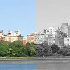
\includegraphics[width=.5\textwidth]{Test Image}
\caption{In the above picture, the left is the training data and the right is the test data}
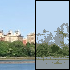
\includegraphics[width=.5\textwidth]{Basic Agent Prediction}
\caption{In the above picture, the left is the training data and the right is the prediction}
\end{figure}
\vfill
\clearpage

\section*{The Improved Coloring Agent}
The improved agent, or Color M.E. Happy (Mesmerizing Execution), functions in a similar way to the basic agent. To improve this agent, however, more color clusters (12 instead of 5) were considered. 3x3 clusters were still used so the agent could have greater accuracery in choosing colors since using 5x5 clusters showed to produce a lower quality image with a larger black border.\\
To improve this agent, there was trial and error pertaining to what the code could handle, as well as, what helped and what ultimately made the image worse (the 3x3 versus 5x5 clusters being an example). This was done to ultimately create the best prediction possible for our code and avoid overfitting.\\
In terms of preprocessing, this was mainly done in Agent.py, which did the conversion of RGB to grayscale and found variance and gradients in our test image, and checked the color predictions of regions.\\
With the improved agent, there is greater definition in the trees, and the buildings have their own color and can be easily discerned from the background. The lake is also more accurate in terms of color.\\
One of the reasons a linear model is a bad idea for colorizing an image is the fact that the data isn't really linear, and shouldn't be treated as such. Since each pixel, in the end, has to be represented by three separate values (RGB), a linear model can't accurately express how all three of these values interact and ultimately affect the final image.\\
Ideally, with all the time, energy, and resources, the improved agent could use a strong parametric model that adjusts what color is chosen based, not only on the training data, but related pixels in the image being processed, so the final result is more comprehensive. Neural networks, as proposed in the project description, could also be used to provide deeper training.
\begin{figure}[t]
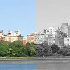
\includegraphics[width=.5\textwidth]{Test Image}
\caption{In the above picture, the left is the training data and the right is the test data}
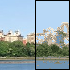
\includegraphics[width=.5\textwidth]{Improved Agent Prediction}
\caption{In the above picture, the left is the training data and the right is the improved prediction}
\end{figure}
\vfill
\clearpage

\end{document}